% TEMPLATE for Usenix papers, specifically to meet requirements of
%  USENIX '05
% originally a template for producing IEEE-format articles using LaTeX.
%   written by Matthew Ward, CS Department, Worcester Polytechnic Institute.
% adapted by David Beazley for his excellent SWIG paper in Proceedings,
%   Tcl 96
% turned into a smartass generic template by De Clarke, with thanks to
%   both the above pioneers
% use at your own risk.  Complaints to /dev/null.
% make it two column with no page numbering, default is 10 point

% Munged by Fred Douglis <douglis@research.att.com> 10/97 to separate
% the .sty file from the LaTeX source template, so that people can
% more easily include the .sty file into an existing document.  Also
% changed to more closely follow the style guidelines as represented
% by the Word sample file. 

% Note that since 2010, USENIX does not require endnotes. If you want
% foot of page notes, don't include the endnotes package in the 
% usepackage command, below.

% This version uses the latex2e styles, not the very ancient 2.09 stuff.
\documentclass[letterpaper,twocolumn,10pt]{article}
\usepackage{usenix,epsfig,endnotes,url}
\begin{document}

%don't want date printed
\date{}

%make title bold and 14 pt font (Latex default is non-bold, 16 pt)
\title{\Large \bf TCP BBR - Assessing Performance in a Data Center Environment}

%for single author (just remove % characters)
\author{
{\rm Colin Howes}\\
University of Waterloo
\and
{\rm Camilo Mu\~{n}oz}\\
University of Waterloo
% copy the following lines to add more authors
% \and
% {\rm Name}\\
%Name Institution
} % end author

\maketitle

% Use the following at camera-ready time to suppress page numbers.
% Comment it out when you first submit the paper for review.
\thispagestyle{empty}


\subsection*{Abstract}

Modern data centers support massively parallel distributed applications that drive products such as web search, social network composition, and targeted advertising. Network protocols supporting these applications must tolerate high intensity many-to-one traffic while providing high throughput and short latencies for update and query traffic. Recent work has endeavoured to improve the performance of TCP in data center environments through modifications to TCP's congestion control mechanisms. Here, we assess the viability of TCP BBR for data center environments. TCP BBR was originally proposed as a general purpose replacement for traditional TCP congestion control mechanisms in wide area networks. We show that TCP BBR has advantages over state-of-the-art TCP Cubic in supporting workloads typical of modern data centers, but exhibits poor fairness when multiple flows converge at a single receiver.

\section{Introduction}

Large-scale web services rely heavily on massively parallel distributed systems, requiring high throughput and short latencies in order to keep background data structures up to date while meeting strict timing requirements \cite{alizadeh_data_2010, chen_understanding_2009, wu_ictcp:_2013}. While these services are diverse, ranging from web search and social network composition to online storage and targeted advertising, they tend to share a common hierarchical design pattern in which aggregators delegate tasks to workers and combine the results before passing data back up through the hierarchy \cite{alizadeh_data_2010, chen_understanding_2009}. 

Data center networks must therefore provide short latencies for bursts of many-to-one traffic converging on a single receiver. In addition, these applications depend on constant updates to underlying data structures in order to provide fresh results, and therefore require high throughput for long-lived background flows \cite{alizadeh_data_2010, chen_understanding_2009, wu_ictcp:_2013}. Given that most data center traffic uses TCP at the transport layer, implementations of TCP used in data centers must be able to accommodate the timing and throughput needs of the applications they support \cite{alizadeh_data_2010}. 

\section{Background}

\subsection{Data Center Workloads}

Modern data centers feature high speed links connecting nodes via low-cost consumer-grade top-of-rack (TOR) switches \cite{alizadeh_data_2010}. These switches typically have small buffers for queued packets, and must support link speeds of 1-100 Gbits/second with round trip times on the order of microseconds to milliseconds \cite{alizadeh_data_2010, chen_understanding_2009}.

The majority of traffic generated in data centers tends to follow a hierarchical \emph{partition/aggregate} pattern, with aggregators delegating jobs to workers and passing a partial result to aggregators higher in the hierarchy \cite{alizadeh_data_2010}. For example, the MapReduce model used in Google's early web search workload is based around ``mappers'' performing sub-tasks and sending results to a ``reducer'', which combines the results and then returns an aggregated result which can be reduced further if necessary \cite{dean_mapreduce:_2004}. Latency in applications following the partition/aggregate pattern is bounded by the \emph{slowest} worker, meaning that data center networks must reliably maintain low round-trip-times even at the high end of the latency distribution. Furthermore, background update flows require high throughput to keep application data up-to-date \cite{alizadeh_data_2010}.

\subsection{Performance Impairments}

TCP was designed to provide fair, reliable communication in wide area networks, where round-trip-times are orders of magnitude longer than in data centers. This was traditionally achieved through the use of an \emph{additive increase, multiplicative decrease} (AIMD) congestion control algorithm, where the send rate is increased linearly until packet loss is detected, at which point the send rate is cut in half. Under this approach, packet queues in the bottleneck switch build up until the switch buffer overflows and packets are dropped, at which point the send rate is reduced drastically, allowing buffers to empty \cite{chiu1989analysis}.

\subsubsection{Buffer Bloat}

The AIMD approach to congestion control is problematic, since it causes \emph{buffer bloat}. That is, send rate is only reduced once loss is detected, meaning that switch buffers are kept consistently full even when the network is not congested. This leads to unnecessarily long queuing delays, which are especially problematic in data center environments where applications have low tolerance for latency, and inherent propagation delay is very low \cite{alizadeh_data_2010, cardwell_bbr:_2016, chen_understanding_2009, wu_ictcp:_2013}. In the context of the partition/aggregate pattern, long-lived background flows keep buffers full, meaning that short-lived query traffic is subject to long queuing delays \cite{alizadeh_data_2010}.

\subsubsection{Incast Congestion}

As a result of the nature of the partition/aggregate paradigm, data center networks must tolerate bursts of synchronized traffic from many senders converging on a single receiver across a shared bottleneck (usually the TOR switch). This \emph{incast congestion} causes switch buffers to quickly overfill, causing high queuing delays, packet loss, and retransmissions, ultimately resulting in throughput collapse and long delays \cite{alizadeh_data_2010, chen_understanding_2009, wu_ictcp:_2013}.

\subsection{Related Work}

Two notable recent projects looking to optimize TCP for data center workloads are Data Center TCP (DCTCP) and Incast Congestion Control for TCP (ICTCP) \cite{alizadeh_data_2010, wu_ictcp:_2013}. Both approaches attempt to keep query latencies low while maintaining high throughput via early rate adaption in response to bottleneck congestion.

\subsubsection{DCTCP}

DCTCP was designed to leverage Explicit Congestion Notification (ECN) packet marking at the switch to determine when queue length exceeds some small threshold, $k$. DCTCP responds to ECN marking by conservatively reducing send rate proportionally to the ratio of marked packets. When $k$ is set appropriately, DCTCP reduces query latency by keeping queue sizes short and preventing buffer bloat, while maintaining high throughput for background flows. The major disadvantage of DCTCP is that DCTCP traffic cannot intermix with traffic using other congestion control mechanisms, and thus internal data center traffic must be isolated from external traffic \cite{alizadeh_data_2010, alizadeh_analysis_2011}.

\subsubsection{ICTCP}

ICTCP makes use of the TCP receive window to throttle incoming connections to perceived available bottleneck bandwidth. The key observation motivating the design of ICTCP is that throughput collapse tends to occur on the last-hop switch before reaching the receiver, which is typically the top-of-rack switch. Thus, the receiver can monitor incoming connections and set its receive window for each connection such that each flow only sends at its fair share of the bottleneck bandwidth. ICTCP is effective at avoiding incast congestion, but tends to under-utilize the bottleneck when the number of senders is small \cite{wu_ictcp:_2013}.

\subsection{TCP BBR}

TCP BBR (\emph{B}ottleneck, \emph{B}andwidth, \emph{R}ound-trip time) was originally designed as a general replacement for traditional TCP congestion control mechanisms, and is currently used in Google services including the Google Cloud Platform, YouTube, and Google's B4 Backbone, which is a large network comprised of commodity switches similar to those typically found in data center networks \cite{cardwell_bbr:_2016, cardwell_tcp_2017}. The design of TCP BBR is based on a proof stating that optimal latency and throughput is achieved when the send rate is exactly equal to available bottleneck bandwidth \cite{kleinrock_power_1979}. That is, if the bottleneck can support $b$ bits/second, sending at speed $s > b$ causes buffers to fill, resulting in high queuing delays and eventually packet loss, whereas if $s < b$, the bottleneck is under-utilized. 

The goal of TCP BBR is to send data as fast as possible without causing queue build up. In order to accomplish this, the BBR algorithm uses measurements of round-trip time and packet delivery rates to estimate available bandwidth and probe for an ideal send rate. Send rate is periodically increased, and if an increase in round-trip time (RTT is observed, it is interpreted as queue buildup and the send rate is throttled back. Conversely, if no change in RTT is observed, this is interpreted as bandwidth under-utilization and send rate is increased further \cite{cardwell_bbr:_2016}.

While testing in Google's services indicates that TCP BBR is able to support lower latency and throughput than TCP Cubic, we are not aware of any work directly assessing the performance of TCP BBR on workloads typical of those in modern data centers \cite{cardwell_tcp_2017, cardwell_bbr:_2016}. 

\section{Experimental Design}

TCP BBR shares some important characteristics with DCTCP and ICTCP. All three mechanisms attempt to reduce latency by proactively adjusting the send rate in response to perceived congestion, keeping buffers small, and reacting conservatively to packet loss. Given these similarities, we hypothesized that TCP BBR would perform well in the data center environments modelled in \cite{alizadeh_data_2010} and \cite{wu_ictcp:_2013}, and might be suitable for adoption in production data centers. 

Here, we examine the performance of TCP BBR in experiments similar to those used in \cite{alizadeh_data_2010} and \cite{wu_ictcp:_2013}, and assess its performance in terms of query latency, throughput, and fairness in comparison with state-of-the art TCP Cubic.

All the experiments presented in this work were conducted using the SYN cluster environment at the University of Waterloo. This environment features six clusters of 16 nodes connected via Mellanox SX1012 top-of-rack switches. Importantly, these switches utilize cut-through switching and lossless ethernet, and as such, do not store packets in buffers as in the traditional top-of-rack switches discussed above. Rather, layer 2 flow control is enforced at the outgoing interface, and packet loss due to network congestion is eliminated entirely \cite{noauthor_mellanox_sx1012, noauthor_mellanox_sx1012_pdf}. All nodes were installed with Ubuntu Linux 14.04.1 LTS. We updated the kernel to Linux 4.13.0, which includes TCP Cubic as the default congestion control algorithm, as well as a production quality implementation of TCP BBR as an optional kernel module.

In order to model query traffic and multiple converging flows, we implemented a simple partition aggregate application in C++ \footnote{source code and data -  https://github.com/chowes/data-center-bbr}. In our application, an aggregator connects to each worker and sends synchronized requests specifying the traffic type along with a transfer size (query tests) or test length (throughput and fairness tests). We also implemented a simple throughput monitoring tool as a replacement for traditional tools that we found to be unsuitable for measuring converging throughput from multiple distinct nodes. Our aggregator is designed using a purely thread based architecture (i.e. thread per connection), which we believe is sufficient for this use case, and is consistent with architectures used in other tools \cite{iperf}. It is worth noting, however, that thread based designs are known to be problematic in production systems handling very large numbers of concurrent connections \cite{pariag2007comparing}.

For query latency and throughput experiments we present mean $\pm 95$ $\%$ Confidence Interval (CI) and cumulative distribution functions (CDF) derived from 100 samples for a given number of worker/sender nodes. We also present the $95^{th}$ percentile of query latency, since this is highly relevant in determining the performance of partition/aggregate applications. Given that transient variance in throughput is essential for characterizing fairness and convergence, we present time series throughput data taken at one second intervals from a single trial, as in past work \cite{alizadeh_data_2010, wu_ictcp:_2013}.

\section{Results}

\subsection{Query Latency}

We assessed query latency using a simple partition/aggregate application that requested a total of 1 MiB from a set of $n \in [1, ..., 40]$ worker nodes, such that the aggregator received $1 / n$ MiB from each of the $n$ workers. We defined response time as the total time to receive all $n$ subqueries. We assessed query delay both in the absence of background traffic and with a single long-lived TCP flow arriving at the aggregator, though due to resource limitations we were only able to test with up to $n = 20$ worker nodes in the presence of a background flow since these tests took significantly longer. 

In the absence of background traffic, we saw no difference between TCP BBR and TCP Cubic in terms of query latency, and did not observe any evidence of incast congestion collapse (Figure 1, Figure 2, Figure 3). However, when we added a background flow arriving at the aggregator, we observed a drastic increase in both mean latency and variance in query latency. Moreover, TCP BBR showed a significant advantage over TCP Cubic in terms of mean and $95^{th}$ percentile latency, especially when the number of workers was small, though performance began to converge at high levels of congestion (Figure 4, Figure 5, Figure 6). 

Thus, in the presence of a background flow, queries over TCP BBR experienced significantly less mean latency, as well as lower $95^{th}$ percentile latency than queries over TCP Cubic. Additionally, the CDF in Figure 6 shows that a greater proportion of queries over BBR exhibited very low latency in the presence of a background flow, though this has little practical value for partition/aggregate applications since job completion time tends to be bounded by tasks at the upper end of the latency distribution.

\begin{figure}
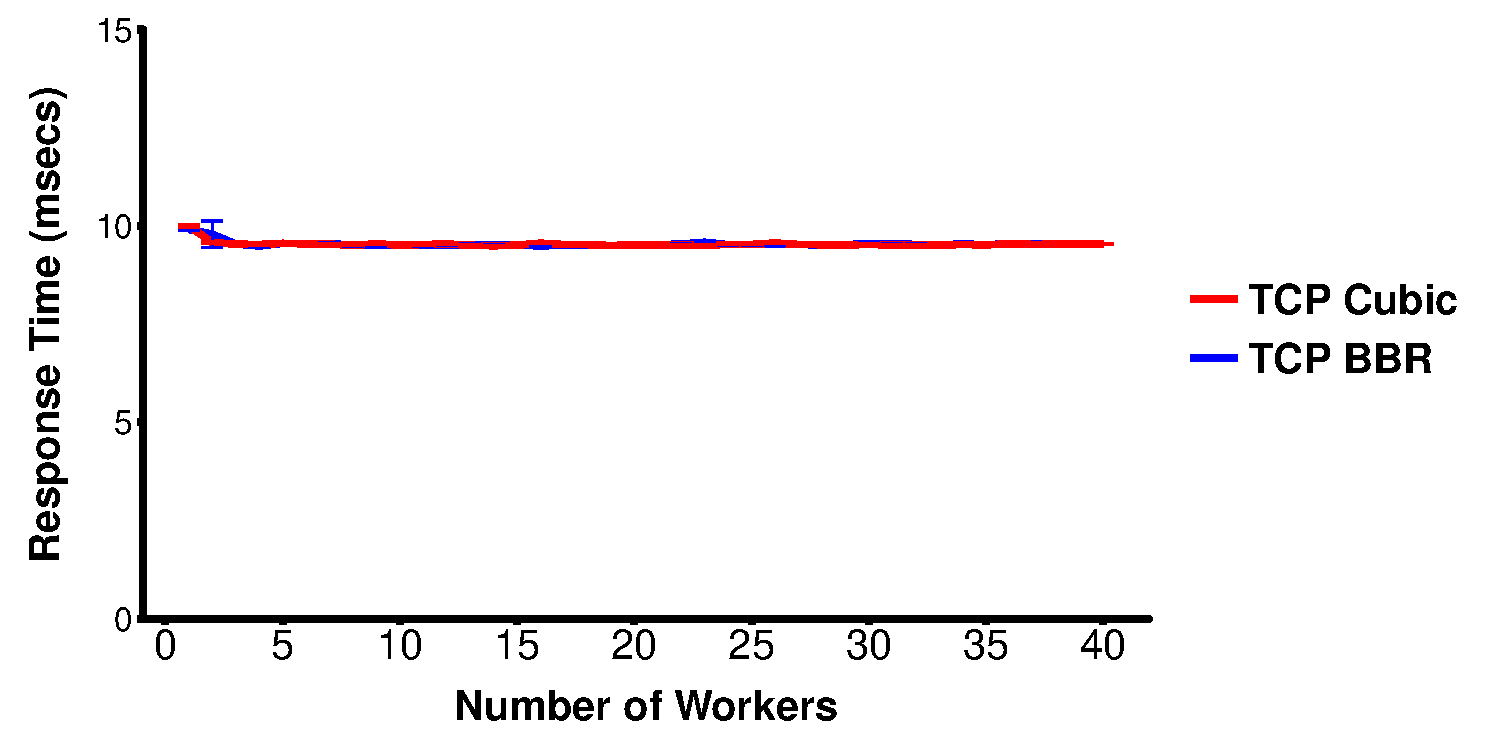
\includegraphics[height=1.6in,width=3.2in]{plots/query_avg.pdf}
\caption{Mean query latency $\pm$ 95 \% CI in the absence of background traffic averaged over 100 samples. Performance is similar between TCP BBR and TCP Cubic.}
\end{figure}

\begin{figure}
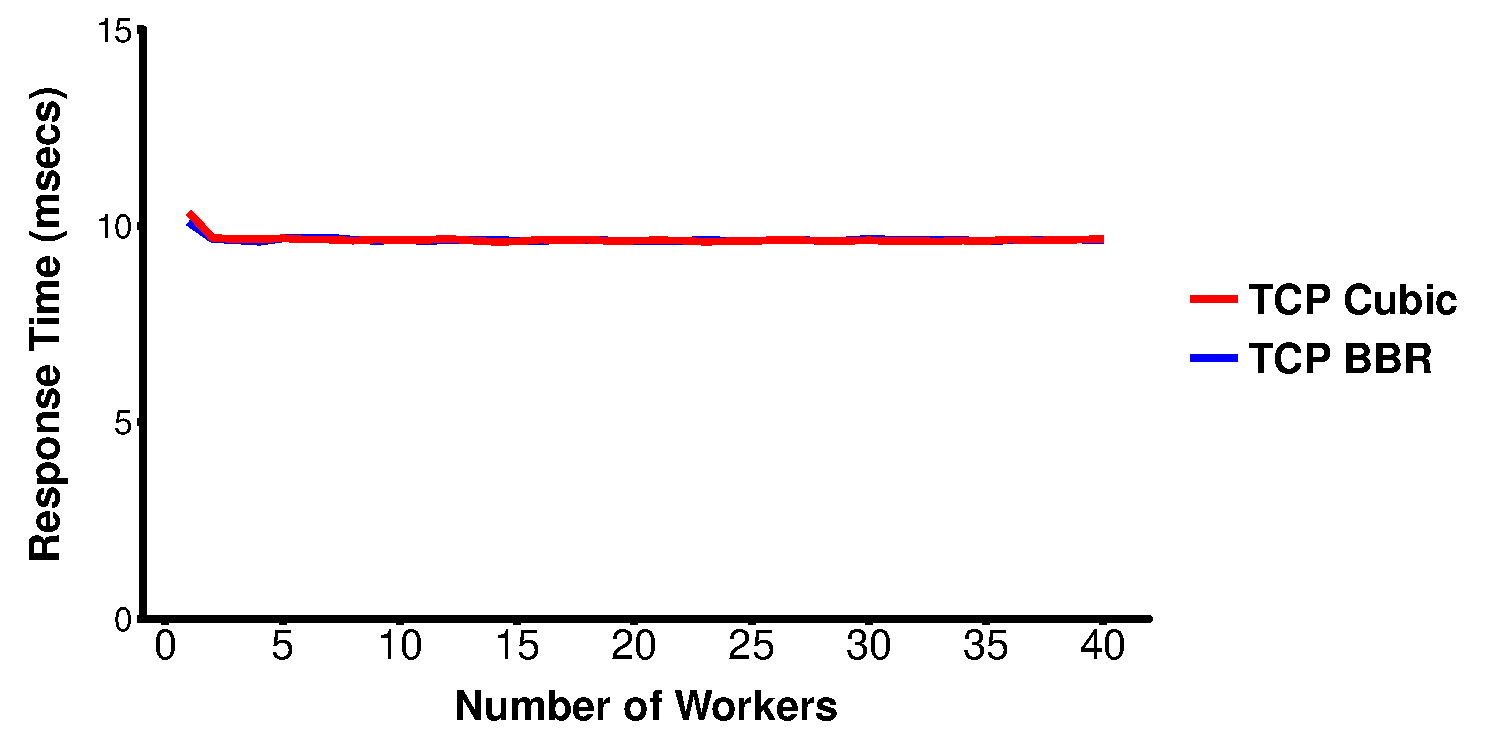
\includegraphics[height=1.6in,width=3.2in]{plots/query_percentile.pdf}
\caption{$95^{th}$ percentile of query latency in the absence of background traffic over 100 samples. Performance is similar between TCP BBR and TCP Cubic.}
\end{figure}

\begin{figure}
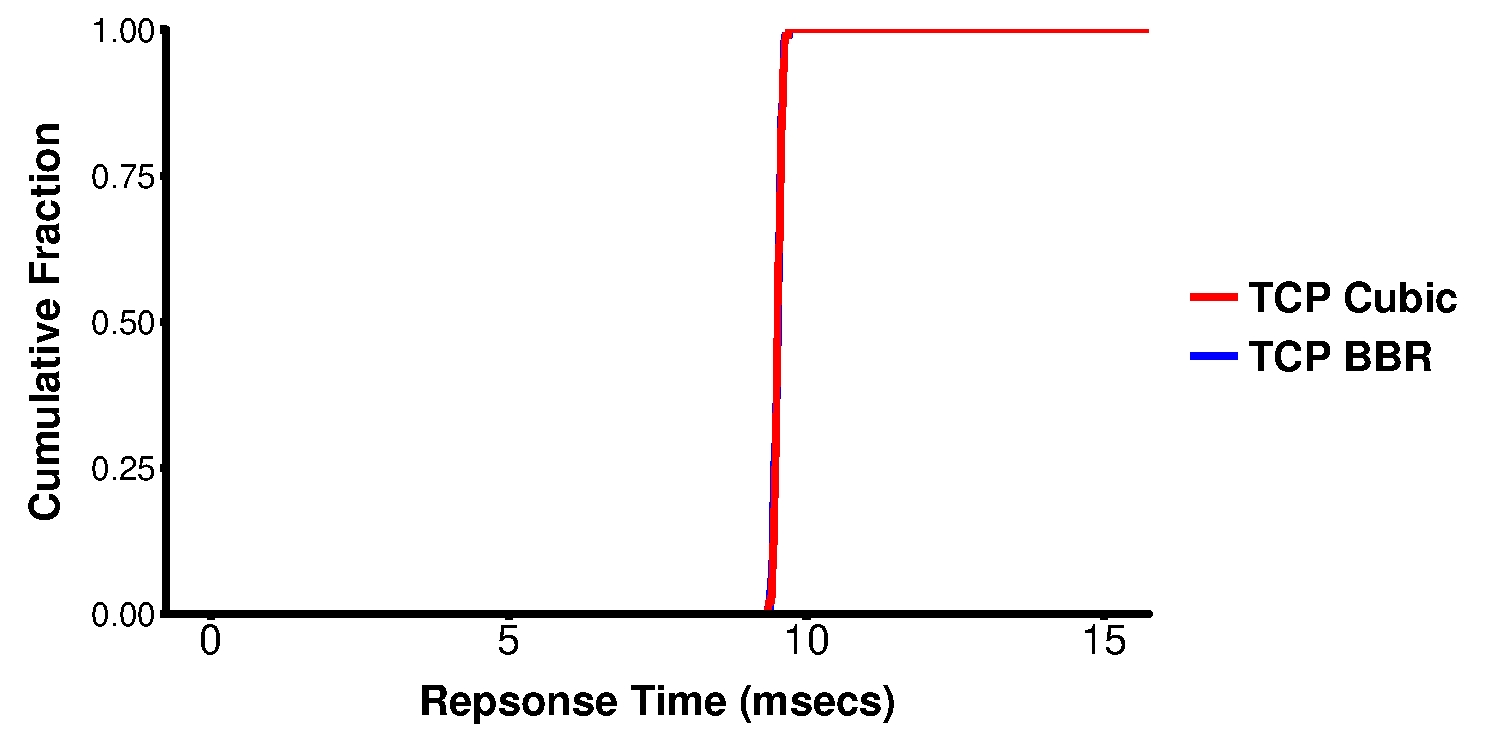
\includegraphics[height=1.6in,width=3.2in]{plots/query_cdf.pdf}
\caption{CDF of query latency in the absence of background traffic over 100 samples when querying from 20 worker nodes. Performance is similar between TCP BBR and TCP Cubic.}
\end{figure}

\begin{figure}
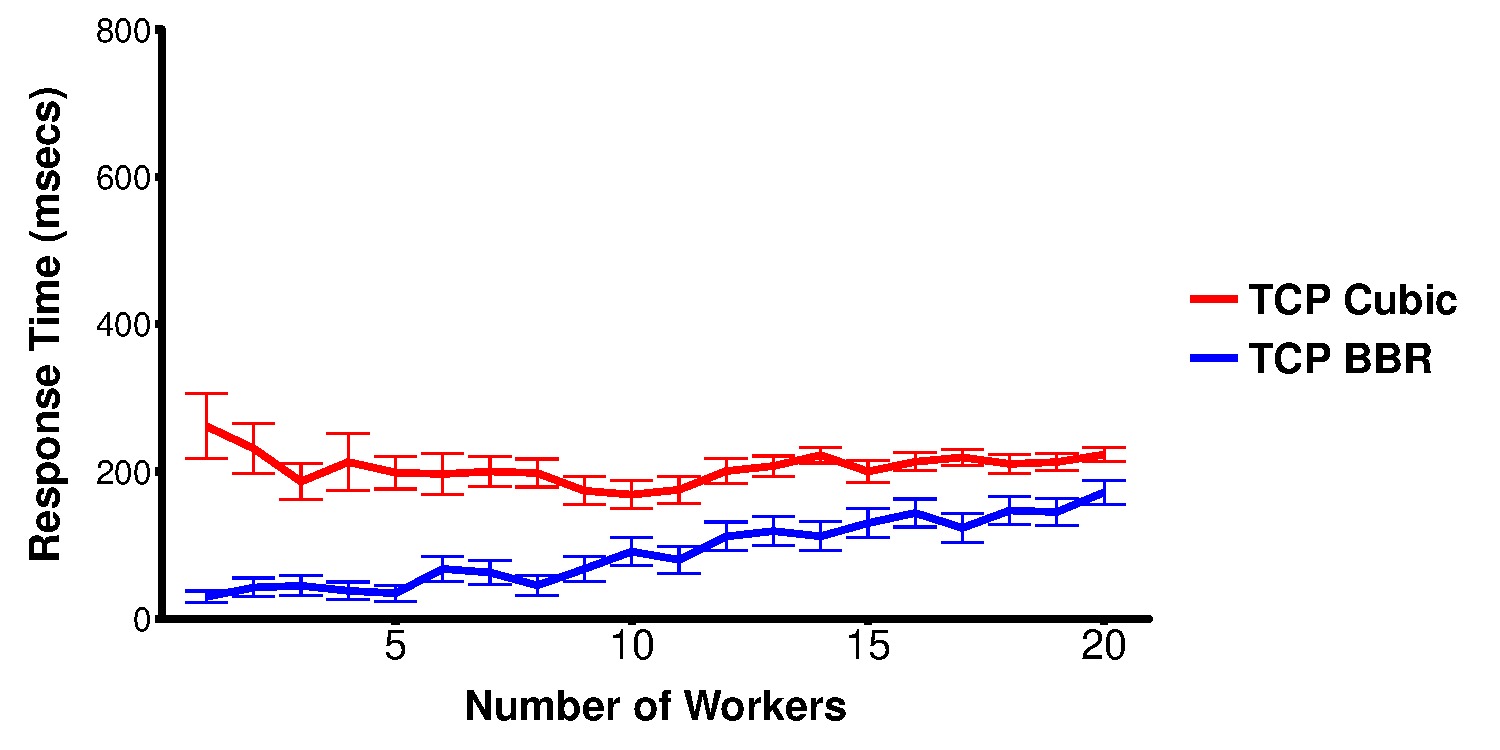
\includegraphics[height=1.6in,width=3.2in]{plots/query_bg_avg.pdf} 
\caption{Mean query latency with a single long-lived background flow $\pm$ 95 \% CI averaged over 100 samples. Mean query latency is significantly shorter for TCP BBR compared with TCP Cubic.}
\end{figure}

\begin{figure}
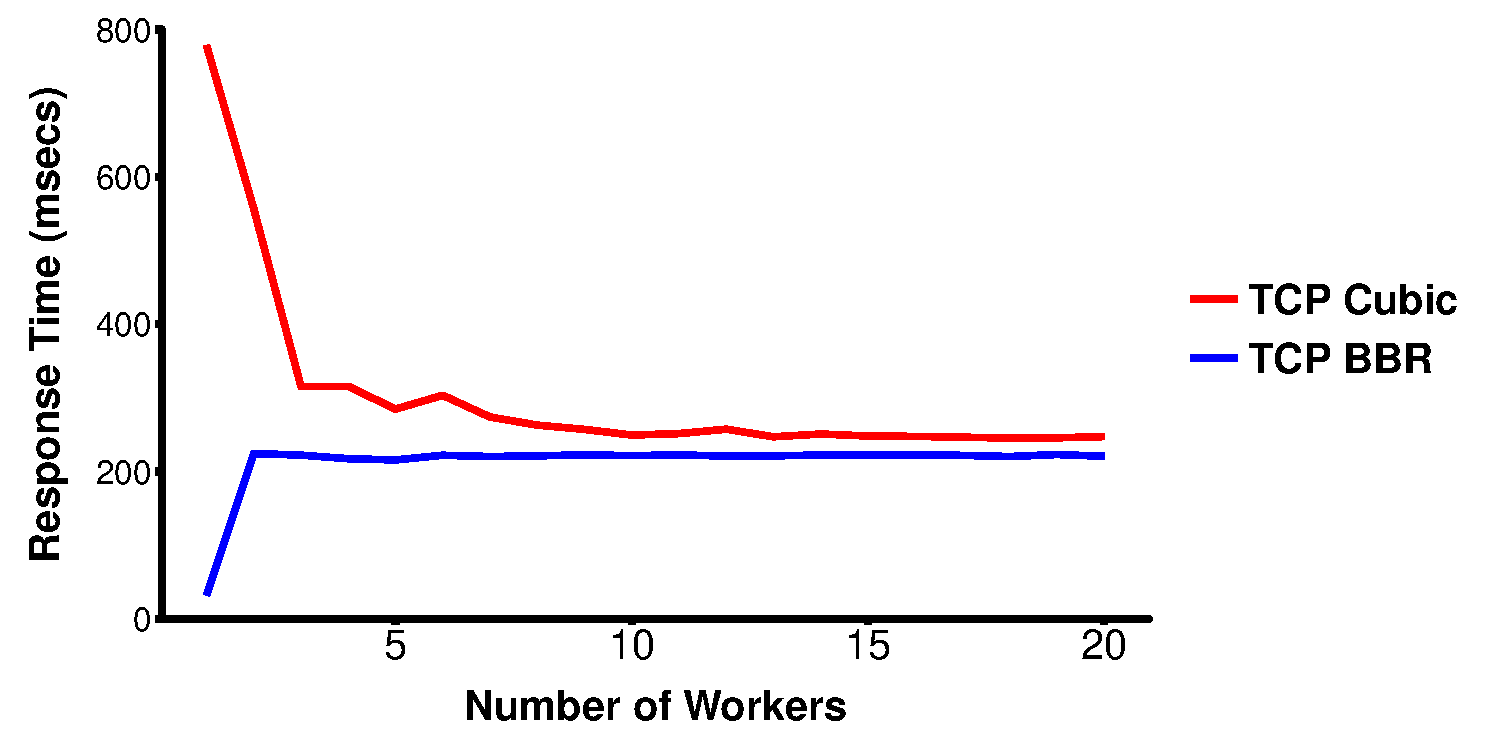
\includegraphics[height=1.6in,width=3.2in]{plots/query_bg_percentile.pdf}
\caption{$95^{th}$ percentile of query latency with a single long-lived background flow over 100 samples. Queries are shorter when using TCP BBR than when using TCP Cubic at the $95^{th}$ percentile of query latency.}
\end{figure}

\begin{figure}
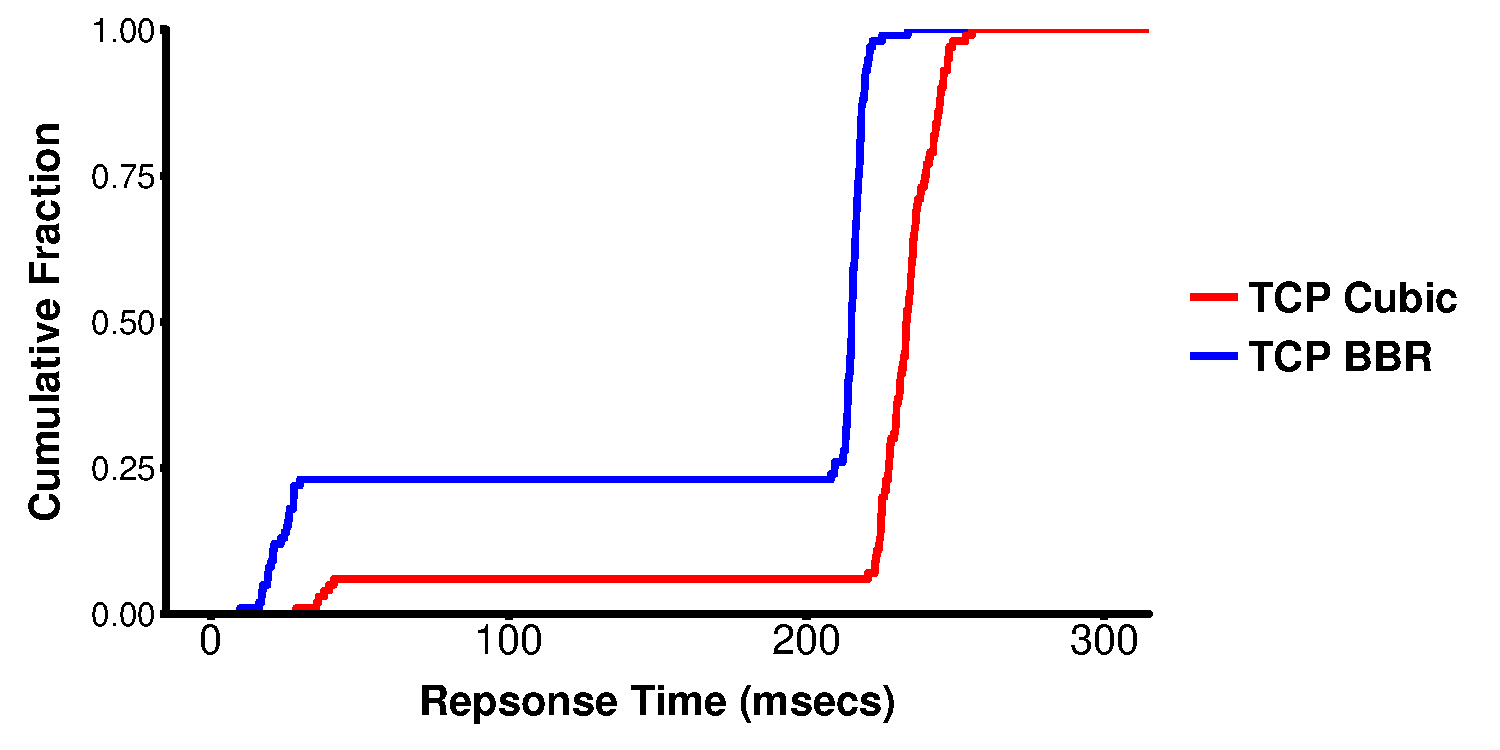
\includegraphics[height=1.6in,width=3.2in]{plots/query_bg_cdf.pdf}
\caption{CDF of query latency with a single long-lived background flow over 100 samples when querying from 20 worker nodes.}
\end{figure}

\subsection{Throughput}

To assess throughput of long-lived flows converging at a single receiver, we started $n \in [1, ..., 20]$ synchronized flows lasting a total of 10 seconds and measured total throughput combined across all flows over the 10 second window. We found that for both TCP BBR and TCP Cubic, throughput decreased as more nodes were added. However, for $n \geq 10$, TCP BBR maintained significantly higher mean throughput than TCP Cubic (see Figure 7). Figure 8 shows the cumulative distribution function of throughput at $n = 20$ converging flows, which indicates that a considerably smaller ratio of TCP BBR flows suffered from decreased throughput due to incast congestion than TCP Cubic, indicating that TCP BBR is more resilient to throughput collapse in incast scenarios. 

\begin{figure}
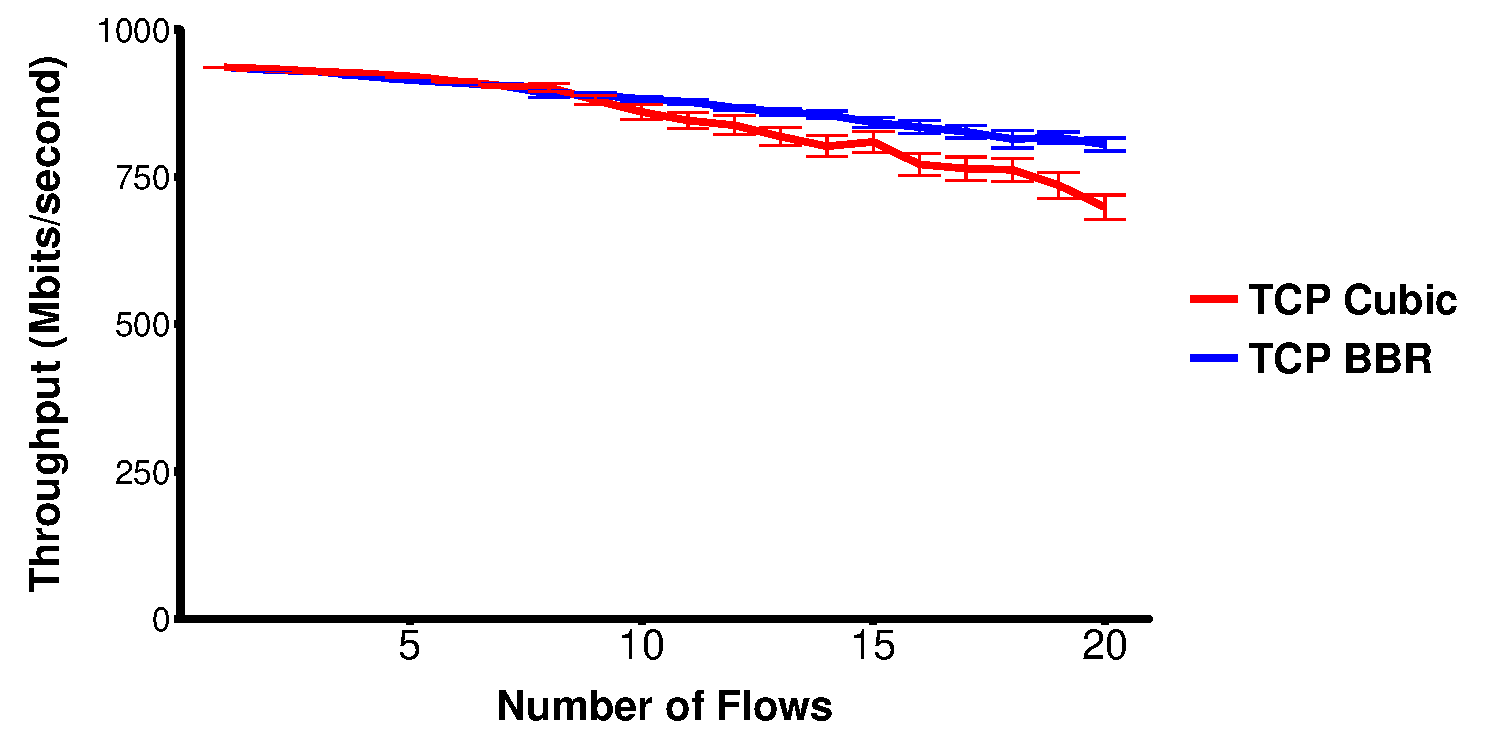
\includegraphics[height=1.6in,width=3.2in]{plots/thru_avg.pdf}
\caption{Mean throughput $\pm 95$ $\%$ CI. Throughput is negatively affected in both TCP Cubic and TCP BBR, though TCP BBR performs significantly better than TCP Cubic for $n \geq 10$.}
\end{figure}

\begin{figure}
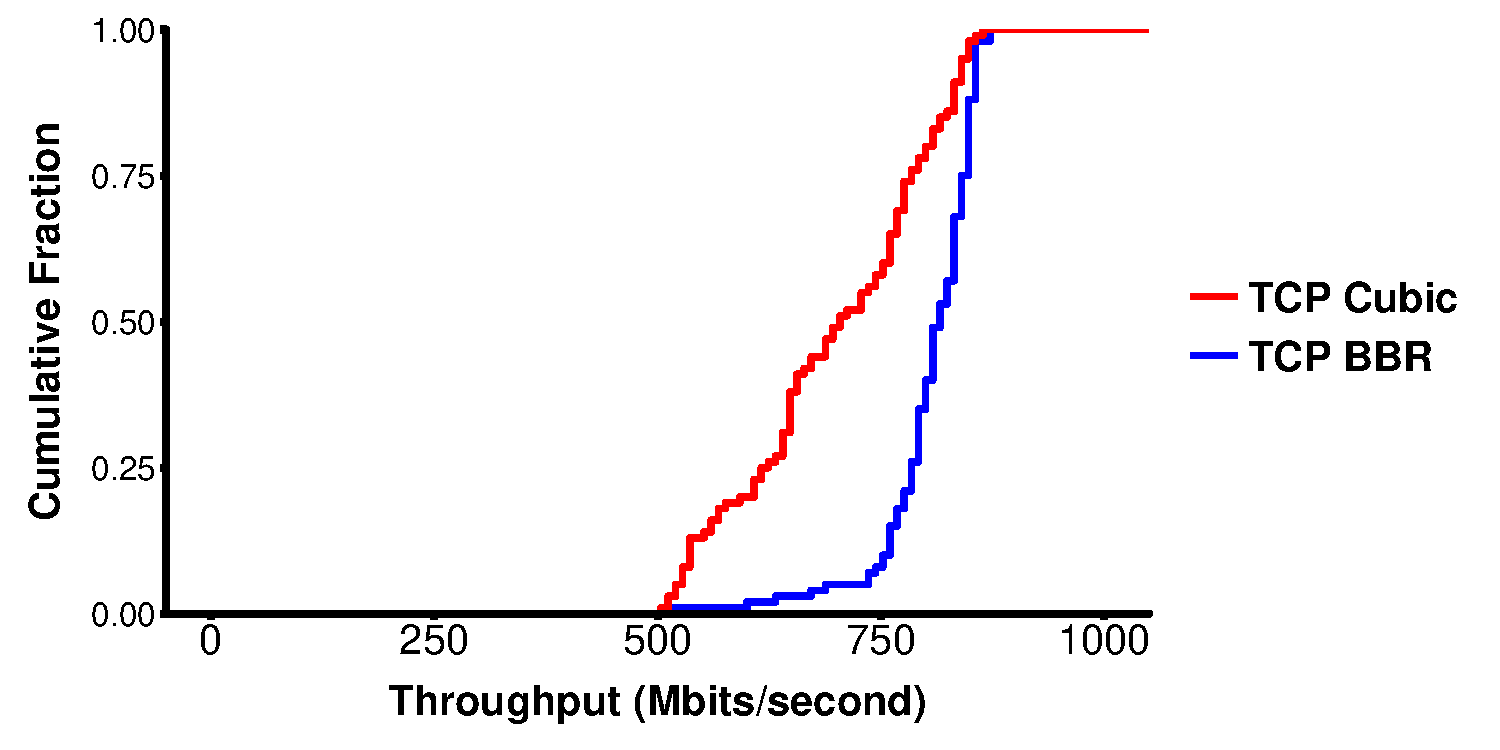
\includegraphics[height=1.6in,width=3.2in]{plots/thru_cdf.pdf}
\caption{CDF of throughput over 100 samples when receiving data from 20 nodes. A smaller fraction of TCP BBR flows are affected by throughput collapse compared to TCP Cubic, where less than half of transfers are able to achieve 75 \% of bottleneck bandwidth.}
\end{figure}

\subsection{Fairness}

In order to evaluate fairness, we measured throughput coming into a single receiver while 5 converging flows originating from separate senders were started and stopped. Each flow was a total of 150 seconds in length, and flow start times were spaced 30 seconds apart. That is, new flows started in 30 second intervals until all 5 flows were transmitting simultaneously, and then each flow stopped in order, spaced 30 seconds apart. If this test were run using a perfectly fair TCP implementation, we would expect to see each flow immediately converge to its fair share of the total bandwidth at each interval. That is, with bottleneck bandwidth $b$ and a total of $n$ flows, we would expect each flow to quickly converge to throughput $b/i$ when $i$ of the $n$ flows are active. 

As shown in Figure 9 and Figure 10, while flows over TCP Cubic converged well, we found that TCP BBR showed poor convergence, with some flows starving completely. This suggests that the advantage shown by TCP BBR in the throughput tests above may be at the expense of fairness, which is undesirable given that each flow may need to constantly maintain high throughput targets. Interestingly, short-lived query traffic does not appear to be adversely affected by this phenomenon, given that we found queries over TCP BBR had significantly shorter overall latency than TCP Cubic even in the presence of background traffic.

\begin{figure}
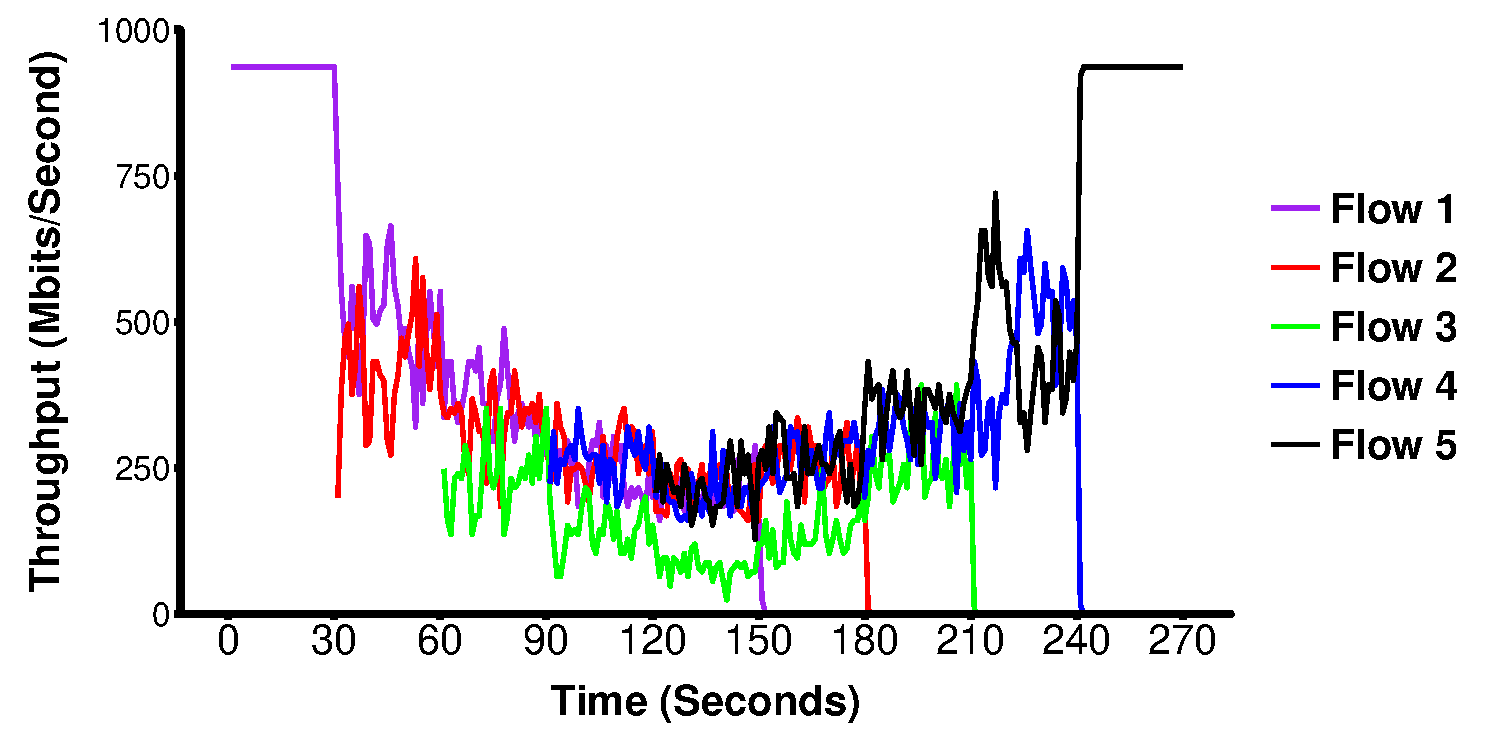
\includegraphics[height=1.6in,width=3.2in]{plots/cubic_converg.pdf}
\caption{TCP Cubic convergence test - 30 second intervals. TCP Cubic converges well as 5 flows are added and removed.}
\end{figure}

\begin{figure}
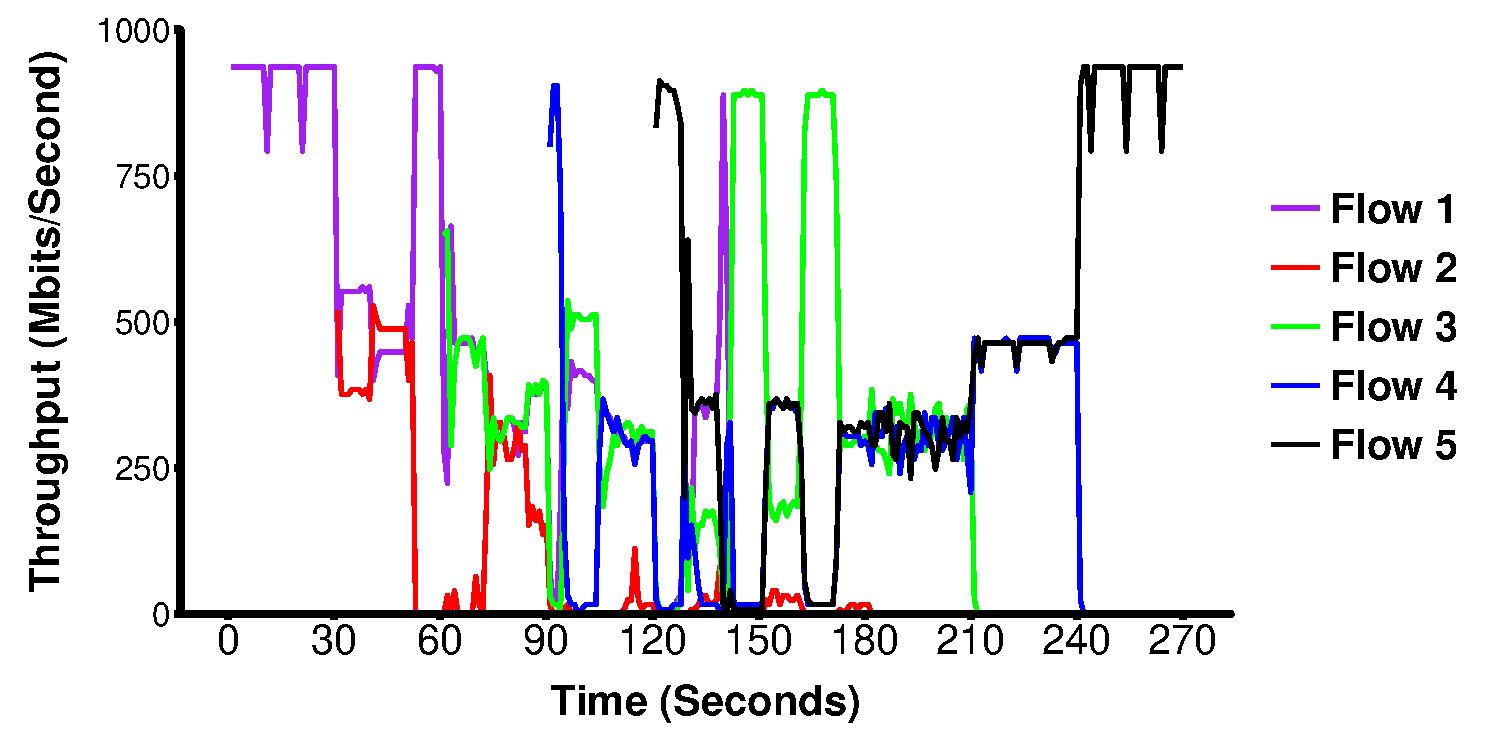
\includegraphics[height=1.6in,width=3.2in]{plots/bbr_converg.pdf}
\caption{TCP BBR convergence test - 30 second intervals. TCP BBR converges poorly, and some flows starve when more than 2 flows share the bottleneck.}
\end{figure}

Our findings are somewhat in agreement with the results obtained in the original TCP BBR paper, which showed that flows take slightly longer than 30 seconds to converge to their fair share of the bottleneck \cite{cardwell_bbr:_2016}. In order to examine whether this is true in our cluster environment, we repeated the test using intervals of 60 seconds and found that flows eventually begin to alternate between sending at full link speed and not sending at all (see Figure 11). 

Given that this is not the intended behaviour of TCP BBR, we suspect that our results were impacted by the use of lossless ethernet and cut-through switching in our cluster, which has its own flow control mechanisms that may be influencing the behaviour of the mechanisms used in TCP BBR \cite{cardwell_bbr:_2016}. It is also possible that TCP rate adjustment algorithm is too aggressive in its throughput adjustments when congestion is high, but round-trip-times remain relatively short compared to in a wide area network.

\begin{figure}
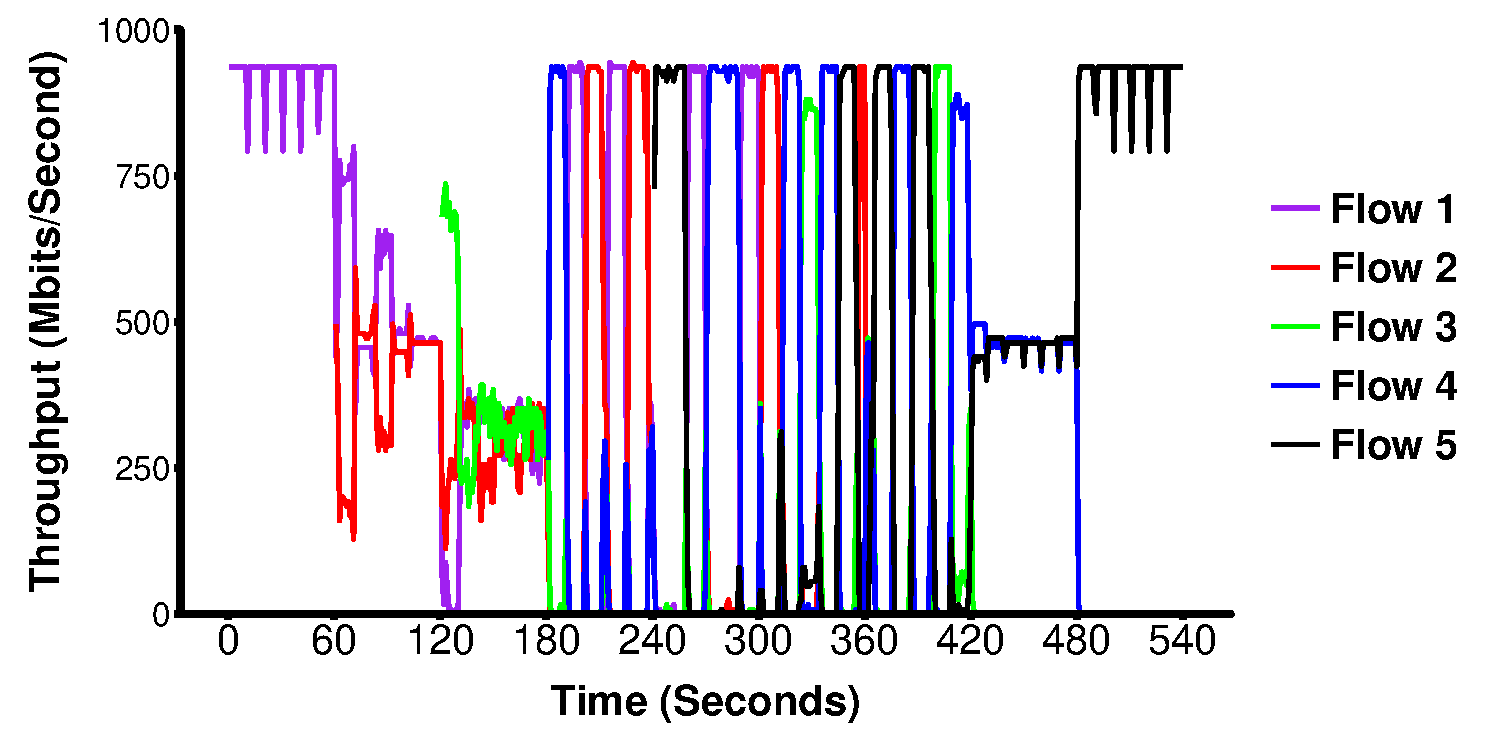
\includegraphics[height=1.6in,width=3.2in]{plots/bbr_converg_long.pdf}
\caption{TCP BBR convergence test - 60 second intervals. TCP BBR converges poorly, and connections oscillate between zero throughput and transmitting at full bottleneck speed when more than 2 flows share the link.}
\end{figure}

\section{Limitations}

We discovered fairly late into our study that the SYN switches use cut-through switching and lossless ethernet rather than the traditional store-and-forward switching mechanisms used in previous evaluations of TCP BBR and TCP congestion control modifications for data center networks \cite{alizadeh_data_2010, cardwell_bbr:_2016, wu_ictcp:_2013}. This difference is fairly significant given that TCP BBR is designed around keeping switch buffers empty in order to reduce queuing delay. We do not have a strong understanding of how layer 2 flow control mechanisms interact with the congestion control mechanisms built into TCP BBR, making this a potential avenue for future research. 

In addition, these differences make it difficult to draw direct comparisons between the work presented here and what has been shown in past work. For example, previous work indicates that TCP New Reno shows high query latency under incast conditions with as few as 10 worker nodes, while we were not able to induce any change in latency in queries over either TCP Cubic or TCP BBR in the absence of background traffic even when querying as many as 40 nodes \cite{alizadeh_data_2010, wu_ictcp:_2013}. This may be due to the improved congestion control mechanisms in Cubic and BBR, but we suspect that we may be observing the effectiveness of layer 2 flow control in these cases.

\section{Conclusions and Future Work}

While we found that TCP BBR has clear advantages over TCP Cubic in terms of query delay and combined throughput when receiving data from multiple senders, the poor convergence of TCP BBR flows indicate that TCP BBR may not be a suitable replacement for TCP Cubic in data center networks. Given that these results are not typical of what has been observed in evaluations of TCP BBR on wide area networks, we suspect that our findings may have been influenced by interactions between flow control mechanisms present in our cluster and TCP BBR's congestion control mechanisms. We believe that these results warrant further investigation in data center networks using traditional store-and-forward switching in order to determine whether TCP BBR simply does not interact well with this method of flow control, or if the BBR algorithm needs to be adjusted for use on low latency, high throughput networks.

Additionally, it would be informative to compare TCP BBR with TCP congestion control mechanisms designed specifically for use in data centers. One of the major drawbacks of DCTCP is that it cannot coexist with conventional TCP traffic, and is therefore only suitable when internal flows can be isolated from traffic from external sources \cite{alizadeh_data_2010}. Since TCP BBR has no such requirements, there is incentive to adopt a general purpose solution for data center use if similar performance can be achieved.

Additionally, given that this study and past work on data center congestion control mechanisms have used simplistic models of query and update traffic, it would be beneficial to assess the performance of these congestion control mechanisms in real world low-latency applications such as high performance computing. This would provide the benefit of concrete ``value added'' data, and could guide the development of more sophisticated workload generators for use in future work.

In summary, we have provided an evaluation of TCP BBR in comparison to state-of-the-art TCP Cubic using workloads characteristic of partition/aggregate applications common in modern data centers. We have shown that TCP BBR has a significant advantage over TCP Cubic in terms of query delay and overall throughput in many-to-one traffic scenarios, but suffers from significant fairness and convergence issues.

\section{Acknowledgements}

We would like to thank Dr. Tim Brecht for his help and guidance throughout the term, as well as Lori Paniak for helping us to get access and set up the environment on the SYN cluster.

{\footnotesize \bibliographystyle{acm}
\bibliography{bbr.bib}}

\end{document}







